\chapter{Convolución}

\section{Definición}
En el presente capítulo, exploramos la operación de convolución, una componente fundamental en la teoría del Análisis de Fourier. En la segunda parte, estudiaremos aplicaciones en el ámbito computacional, donde por ejemplo el filtrado de imágenes es gobernado por esta operación, y el uso del Teorema de Convolución que será sin lugar a duda el eje central del trabajo. 

\begin{definicion}
Sean $f,g  \in \mathscr{L}^0(\mathbb{R}^n)$. Dado $x \in \mathbb{R}^n$, decimos que la \textit{convolución} está definida en $x\in \mathbb{R}^n$ si se cumple la condición 
\begin{equation}
    \int_{\mathbb{R}^n} |f(x-y)g(y)| \, dy < \infty,
\end{equation}
En esa situación, se establece la definición
\begin{equation}
    (f*g)(x) = \int_{\mathbb{R}^n} f(x-y)g(y) \, dy < \infty.
\end{equation}
\end{definicion}

\begin{observacion}
  El concepto de convolución tiene perfecto sentido en funciones definidas c.p.d. en $\mathbb{R}^n$, ya que el valor de la convolución (cuando proceda) de dos funciones en un punto es completamente independiente de las posibles alteraciones de estas en conjuntos de medida nula.
\end{observacion}

\noindent A continuación, probaremos que si $f,g \in \mathscr{L}^1(\mathbb{R}^n)$, entonces la convolución está definida para todo punto en $\mathbb{R}^n$.

\begin{lema}\label{lema_gamma}
   Sean $f,g \in \mathscr{L}^0(\mathbb{R}^n)$. La función $\gamma : \mathbb{R}^{n+n} \rightarrow \mathbb{C}$ con
    \begin{equation}
        \gamma(x,y) = f(x-y)g(y) \quad \forall x,y \in \mathbb{R}^n.
    \end{equation}
    es medible.
\end{lema}
\begin{proof}
\noindent Se definen las funciones $f_1,g_2: \mathbb{R}^{n+n} \rightarrow \mathbb{C}$ como
\begin{equation}
    f_1(x,y) =f(x) \quad g_2(x,y) =g(y) \quad \forall x,y \in \mathbb{R}^n.
\end{equation}
Por otro lado, se define la biyección lineal $\phi : \mathbb{R}^{n+n} \rightarrow \mathbb{R}^{n+n}$ por:
\begin{equation}
    \phi(x,y) = (x-y,y) \quad x,y \in \mathbb{R}^n.
\end{equation}

\noindent Se observa que $\gamma = (f_1g_2) \circ\phi$. Luego la medibilidad de $\gamma$ se reduce a probar que las funciones $f_1$ y $g_2$ lo son.
En efecto, dado $A \in \mathcal{B}(\mathbb{C})$, se sigue que
\begin{equation}\label{eq:1}
    (f_1)^{-1} = (f)^{-1}(A) \times \mathbb{R}^n,
\end{equation}
\begin{equation}\label{eq:asd2}
    (g_2)^{-1} =  \mathbb{R}^n \times (g)^{-1}(A).
\end{equation}

\noindent Usando que $f,g$ son funciones medibles, se tiene que~\eqref{eq:1} y~\eqref{eq:asd2} son conjuntos medibles. Llegamos así a la medibilidad de $f_1,g_2$ y por tanto también a la de $\gamma$.
\end{proof}

\begin{teorema}\label{teo:conv}
Sean $f,g \in \mathscr{L}^1(\mathbb{R}^n)$. Entonces se tiene que 
\begin{enumerate}
    \item $f*g$ está definida c.p.d en $\mathbb{R}^n$,
    \item $f*g \in \mathscr{L}^1(\mathbb{R}^n)$ y además se cumple la desigualdad
    \begin{equation}
        ||f*g||_1 \leq ||f||_1 ||g||_1.
    \end{equation}  
\end{enumerate}
\end{teorema}

\begin{proof}
    Consideramos la función $\gamma$ definida en el Lema \ref{lema_gamma}, medible.
    A continuación, probamos que 
    \begin{equation}
        \int_{\mathbb{R}^{n+n}} |\gamma(x,y)| d(x,y) = ||f||_1||g||_1 < \infty.
    \end{equation}

\noindent Para ello observamos que 
\begin{equation}
    \int_{\mathbb{R}^n}\int_{\mathbb{R}^n} |\gamma(x,y)| \, dx \, dy = \int_{\mathbb{R}^n} |g(y)|\int_{\mathbb{R}^n} |f(x-y)| \, dx \, dy  = \int_{\mathbb{R}^n} |g(y)||f||_1 \, dy  = ||f||_1||g||_1.
\end{equation}

\noindent Aplicando el Teorema de Tonelli, se tiene que 
\begin{equation}
        \int_{\mathbb{R}^{n+n}} |\gamma(x,y)| d(x,y) = \int_{\mathbb{R}^n}\int_{\mathbb{R}^n} |\gamma(x,y)| \, dx \, dy = ||f||_1||g||_1 < \infty.
\end{equation}

\noindent Por el Teorema de Fubini, se sigue ahora que:
\begin{itemize}
    \item Para casi todo $x \in \mathbb{R}^n$, la función $y \mapsto \gamma(x,y)$ es integrable en $\mathbb{R}^n$.

    \item La función $x \mapsto\int_{\mathbb{R}^n}\gamma(x,y) \, dy$ definida c.p.d en $\mathbb{R}^n$ es integrable en  $\mathbb{R}^n$.
\end{itemize}

\noindent Por lo que $f*g$ es integrable en $\mathbb{R}^n$, y se tiene que 
\begin{align}
||f*g||_1 &= \int_{\mathbb{R}^n}|(f*g)(x)| \, dx \leq \int_{\mathbb{R}^n}\int_{\mathbb{R}^n}|\gamma(x,y)|\, dy\, dx \\
&= \int_{\mathbb{R}^n}\int_{\mathbb{R}^n}|\gamma(x,y)|\, dx\, dy = ||f||_1||g||_1. \qedhere
\end{align}
\end{proof}


\section{Teorema de Convolución}
\noindent A continuación, probaremos el teorema que servirá de eje central para alcanzar el objetivo propuesto en el presente trabajo. Podemos afirmar, en términos coloquiales, que la Transformada convierte la convolución en el producto. En la segunda parte de la memoria, nos centraremos en aprovechar esta conversión para expresar la convolución entre imágenes como productos puntuales, reduciendo la complejidad computacional considerablemente.
\vspace{-0.07cm}
\begin{teorema} \label{teo}(Teorema de Convolución). Sean $f,g \in \mathscr{L}^1(\mathbb{R}^n)$. Entonces se tiene que 
\begin{equation}
    \widehat{(f*g)}(y) = \widehat{f}(y) \widehat{g}(y) \quad \forall y \in \mathbb{R}^n.
\end{equation}
    
\end{teorema}

\begin{proof}
Sea  $\gamma$ la función introducida en (\ref{lema_gamma}) y  $z \in \mathbb{R}^n$. La función $(x,y) \mapsto \gamma(x,y)e^{-2\pi i \langle x, z \rangle} \, $ es
\begin{itemize}[itemsep=0.5ex,parsep=0pt,topsep=0pt,partopsep=0pt]
    \item  medible en $\mathbb{R}^n \times \mathbb{R}^n$,
    \item integrable en $\mathbb{R}^n \times \mathbb{R}^n$ ya que:
    \begin{equation}
    \int_{\mathbb{R}^{n+n}}  |\gamma(x,y)e^{-2\pi i \langle x, z \rangle}| \, d(x,y) = \int_{\mathbb{R}^{n+n}}|\gamma(x,y)| \, d(x,y) < \infty.
    \end{equation}
\end{itemize}
 Aplicamos entonces el Teorema de Fubini y obtenemos:
\begin{equation*}
\begin{split}
\widehat{(f*g)}(z) &= \int_{\mathbb{R}^n}(f*g)(x)e^{-2\pi i \langle x, z \rangle} \, dx \\
&= \int_{\mathbb{R}^n}\left( \int_{\mathbb{R}^n}  (f(x-y)g(y) \, dy \,e^{-2\pi i \langle x, z \rangle} \right) \, dx \\
&= \int_{\mathbb{R}^n}\int_{\mathbb{R}^n}(f(x-y)g(y)\,  \, e^{-2\pi i \langle x, z \rangle} e^{-2\pi i \langle y, z \rangle}e^{2\pi i \langle y, z \rangle} \, dy  \, dx \\
&= \int_{\mathbb{R}^n}\left(\int_{\mathbb{R}^n}\left((f(x-y)\,  \, e^{-2\pi i \langle (x-y), z \rangle} \,\right) dx \, g(y)e^{-2\pi i \langle y, z \rangle} \,\right) dy  \\
&=  
\int_{\mathbb{R}^n}f(x)\,  \, e^{-2\pi i \langle x, z \rangle} \, dx \, \int_{\mathbb{R}^n}g(y)e^{-2\pi i \langle y, z \rangle} \, dy  \\
&=  
\widehat {f}(z)\widehat{g}(z).  \qedhere
\end{split} 
\end{equation*}
    
\end{proof}



\noindent El Teorema de Convolución permite en el ámbito discreto interpretar el filtrado de imágenes en términos de frecuencias, ya que este se puede ver como el producto puntual de las representaciones de dichas imágenes en el dominio de la frecuencia. Esto proporciona  una mayor explicabilidad acerca del resultado obtenido tras el filtrado. 

\noindent Por ejemplo, imagínese que tratamos de eliminar el ruido de una imagen. Esto en la práctica se puede hacer realizando la convolución de la imagen con un núcleo gaussiano $G_{\sigma}$. Pero si queremos pensar en términos de la frecuencia podemos realizar la operación de convolución usando el Teorema \ref{teo}. Al calcular la Transformada de Fourier Discreta de la imagen, obtenemos su representación en el dominio de la frecuencia. Por otro lado, al calcular la Transformada de Fourier del núcleo gaussiano, obtenemos otro núcleo gaussiano $G_{\sigma'}$, que al multiplicar punto a punto con la Trasformada de la imagen,
elimina aquellas frecuencias altas (las multiplica por cero), al ser un filtro de paso bajo. Por lo que al destransformar el resultado, obtenemos la imagen sin ruido. 

\vspace{0,5cm}
\noindent Este teorema  no solo es relevante en el ámbito computacional. Sin ir más lejos, tiene aplicaciones directas dentro del Análisis de Fourier.
Este puede resultar especialmente útil en la resolución de ecuaciones que involucran la convolución, como ilustraremos en el siguiente ejemplo.

\begin{ejemplo}
    Supongamos $f \in \mathscr{L}^1(\mathbb{R}^n)$ satisface la ecuación
    \begin{equation}\label{eq:ejemplo}
    2024f*f*f*f+f*f*f-2f*f+f = 0 \, \, c.p.d. \, \,\text{en}\, \, \mathbb{R}^n.
    \end{equation}
    Entonces se tiene que $f = 0 \,$ c.p.d.  en $ \mathbb{R}^n$.                                    
\end{ejemplo}
\noindent \textit{Resolución.} 
Suponemos que existe $f \in \mathscr{L}^1(\mathbb{R}^n)$ tal que satisface la ecuación \eqref{eq:ejemplo}. Por el Teorema de Convolución sabemos que
\begin{equation}
    0 = (2024f*f*f*f+f*f*f-2f*f+f) \,\, \widehat{} \; = 2024\widehat{f}(y)^4+\widehat{f}(y)^3-2\widehat{f}(y)^2+\widehat{f}(y) \quad \forall y  \in \mathbb{R}^n.
\end{equation}
Tenemos así que $\widehat{f}\left(\mathbb{R}^n\right) \subset \mathcal{Z}$, donde
\begin{equation}
    \mathcal{Z} = \{0,w_1,w_2,w_3\}, \quad w_1,w_2,w_3 \in \mathbb{C}.
\end{equation}
Como $\widehat{f}$ es una función continua, y $\mathbb{R}^n$ es conexo, se concluye que $\widehat{f}(\mathbb{R}^n)$ es un subconjunto conexo de $\mathcal{Z}$. Como los únicos subconjuntos conexos de  $\mathcal{Z}$ son los conjuntos que contienen un único punto, concluimos que $\widehat{f}$ es constante, y se cumple una de las siguientes opciones: 
\begin{itemize}
    \item $\widehat{f}=0$.
    \item $\widehat{f}=w, \quad  w \in \{w_1,w_2,w_3\}$.
\end{itemize} 


\noindent No obstante, de acuerdo con el Lema de Riemann-Lebesgue, necesariamente
$\underset{\substack{||y|| \rightarrow \infty}}{\lim}\widehat{f}(y)=0.$
Esto nos lleva a deducir que la única alternativa es que  $\widehat{f}(y) = 0 \, \, \forall y \in \mathbb{R}^n$.
El Teorema de Unicidad asegura por tanto que $f=0 \, \, c.p.d$. Es interesante observar que si 
\begin{equation}\label{eq:ejemplo}
    2024f*f*f*f+f*f*f-2f*f+f = 0 \, \, p.d. \, \, \text{en}\, \, \mathbb{R}^n,
\end{equation}
se concluye que  $f=0 \,$ p.d. en $\mathbb{R}^n$. En efecto, de lo razonado anteriormente, se tendría que $f=0 \, \, c.p.d$. Lo cual implicaría que los términos donde aparece la operación de convolución están definidos en todo punto y son idénticamente nulos. Por lo que  se tendría 
\begin{equation}
    f(x) = -(2024f*f*f*f)(x)-(f*f*f)(x)+(2f*f)(x) = 0\, \, p.d. \, \, \text{en}\, \, \mathbb{R}^n.
\end{equation}

\begin{observacion}
En la mayoría de textos que abordan la convolución para su aplicación en el ámbito computacional encontramos tras este teorema la fórmula $\widehat{fg} = \widehat{f}*\widehat{g}$. De manera que se sugiere que la Transformada convierte la operación de convolución en el producto y viceversa. Así, la convolución en el dominio del tiempo se transforma en el producto en el dominio de la frecuencia, y la multiplicación en el dominio del tiempo corresponde a la convolución en el dominio de la frecuencia. Puede por tanto extrañar que esta no aparezca en esta sección.
Sin embargo, es importante destacar que si $f$ y $g$ pertenecen al espacio de las funciones integrables $\mathscr{L}^1(\mathbb{R}^n)$, el producto puntual $fg$ no necesariamente pertenece a $\mathscr{L}^1(\mathbb{R}^n)$.  Y por tanto, ahora mismo no podemos abordar esta cuestión. 
No obstante, esta ecuación se retomará en un contexto diferente más adelante. Una vez que cambiemos el marco de trabajo adecuadamente esta tomará pleno sentido.

\end{observacion}


\section{Propiedades de la convolución}


\noindent Terminaremos el capítulo probando algunas propiedades de la convolución. La demostración de estas proposiciones será inmediata empleando el Teorema de Convolución, lo que subraya nuevamente su importancia.

\begin{observacion}
    Las igualdades que aparecen en la siguiente proposición son casi por doquier en $\mathbb{R}^n$.
\end{observacion}


\begin{proposicion}\label{prop:conv}
    Sea $f,g,h \in \mathscr{L}^1(\mathbb{R}^n)$ y sea $\alpha \in \mathbb{C}.$ Entonces se tiene que
    \begin{itemize}
        \item $f*g = g*f$,
        \item $(f+g)*h = f*h + g*h$,
        \item $(\alpha f)*h = \alpha(f*h), $
        \item $(f*g)*h = f*(g*h)$.
    \end{itemize}
\end{proposicion}

\begin{proof}
    Por un lado el Teorema \ref{teo} nos permite trasladar las operaciones conmutativa y distributiva de la convolución a la de los números complejos vía la Transformada de Fourier. Seguidamente el Teorema de Unicidad nos proporciona las igualdades casi por doquier correspondientes.
\end{proof}


\noindent Proporcionaremos al lector una breve motivación acerca del siguiente resultado que puede pasar inadvertida. La proposición \ref{prop} (que llevaremos más adelante al ámbito discreto) es crucial en el contexto de las redes convolucionales. Esta es conocida como la \textit{equivariancia de la traslación}, la cual expresa que si trasladamos una imagen y realizamos la convolución obtenemos el mismo resultado que si trasladamos la imagen convolucionada. Su importancia reside en que un objeto de una imagen no tiene por qué estar fijo para que pueda ser detectada por una \textit{CNN} (Red neuronal convolucional); el sistema funciona de la misma manera en diferentes ubicaciones, pero su respuesta cambia a medida que varía la ubicación del objetivo. Por tanto, la red no necesita aprender diferentes representaciones para objetos ubicados en diferentes partes de la imagen.

\begin{proposicion} \label{prop}Sea $f \in \mathscr{L}^1(\mathbb{R}^n)$ y sea $t \in \mathbb{R}^n.$ Entonces \begin{equation}\label{eq:prop}
    \tau_t(f*g)= \tau_t(f)*g = f*\tau_t(g).
\end{equation} 
\end{proposicion}

\begin{proof}
Usando la proposición \ref{prop:tras}, obtenemos
\begin{equation}
    \widehat{\tau_t(f*g)}(y) = e^{-2 \pi i \langle t, y \rangle}\widehat{(f*g)}(y) = e^{-2 \pi i \langle t, y \rangle}\widehat{f}(y)\widehat{g}(y) =\widehat{\tau_tf}(y)\widehat{g}(y) =  
    (\tau_t(f)*g) \,\,\widehat{}\,\,(y).
\end{equation}  
Posteriormente, el Teorema de Unicidad asegura la primera igualdad de~\eqref{eq:prop}. Para la segunda basta con intercambiar $f$ y $g$.
\end{proof}



\begin{proposicion}
     Sea $f,g \in \mathscr{L}^1(\mathbb{R}^n)$. Entonces 
     \begin{itemize}
         \item $\overline{f*g}=\overline{f}*\overline{g},$
         \item $\widetilde{f*g}=\widetilde{f}*\widetilde{g},$
         \item ${\overline{\widetilde{(f*g)}}}(y) = {\overline{\widetilde{(f)}}}\,\,{\overline{\widetilde{(g)}}}.$
     \end{itemize}
\end{proposicion}
\begin{proof}
    La prueba es inmediata usando el Teorema \ref{teo} y el Teorema de Unicidad.
\end{proof}

\begin{proposicion}
     Sean $f,g \in \mathscr{L}^1(\mathbb{R}^n)$, y $a \in \mathbb{R}^+$. Entonces 
     \begin{equation}\label{eq:prop2}
         H_a(f*g) = a^{-n}(H_af)*(H_ag).
     \end{equation}
\end{proposicion}

\begin{proof}

\begin{equation}
    \widehat{H_a(f*g)} = \frac{1}{a^n}\widehat{(f*g)}\left(\frac{1}{a}\right) = \frac{1}{a^n}\widehat{f}\left(\frac{1}{a}\right)\widehat{g}\left(\frac{1}{a}\right). 
\end{equation}
\begin{equation}
    (a^n(H_af)*(H_ag))\, \, \widehat{} = a^n\widehat{H_af}\widehat{H_ag} = a^n\frac{1}{a^n}\widehat{f}\left(\frac{1}{a}\right)\frac{1}{a^n}\widehat{g}\left(\frac{1}{a}\right) = \widehat{f}\left(\frac{1}{a}\right)\frac{1}{a^n}\widehat{g}\left(\frac{1}{a}\right).
\end{equation}
Usando el Teorema de Unicidad, concluimos~\eqref{eq:prop2}.
\end{proof}


\begin{definicion}
Sean $f,g \in \mathscr{L}^1(\mathbb{R}^n)$. Denominaremos correlación de $f,g$ a la operación $f \star g$ dada por 
\begin{equation}
     (f \star g)(x) = \int_{\mathbb{R}^n} \overline{f(y)}g(x+y)\, dy \quad \text{para los x} \in \mathbb{R}^n \,\text{en los que tenga sentido} .
\end{equation}
\end{definicion}

\begin{proposicion}
Sea $f,g \in \mathscr{L}^1(\mathbb{R}^n)$. Entonces $(f \star g)$ está definida $c.p.d$ en $\mathbb{R}^n$ y además se tiene que
\begin{equation}
  (f \star g)(x) = (\overline{\widetilde{f\vphantom{g}}}\ast g)(x).
\end{equation}
\end{proposicion}
\begin{proof}

Por el Teorema \ref{teo:conv}, la convolución está definida c.p.d en $\mathbb{R}^n$. Tomamos un punto $x \in \mathbb{R}^n$ para el que está definida. Entonces se sigue que
\begin{equation}
(\overline{\widetilde{f\vphantom{g}}}\ast g)(x) =  \int_{\mathbb{R}^n} \overline{f(y-x)}g(y) \,dy =  \int_{\mathbb{R}^n} \overline{f(y)}g(y+x) \,dy = (f \star g)(x).
\end{equation}

\noindent Por tanto, $(f \star g)$ está definida $c.p.d$ en $\mathbb{R}^n$ y cumple la igualdad indicada.
\end{proof}

\noindent En la segunda parte de la memoria, proporcionaremos una expresión equivalente para el marco discreto. 
En este, se dice que la convolución entre un núcleo (filtro) $k$ y una imagen $I$ es realizar la correlación con el núcleo invertido $\widetilde{k}*I$ (ya que la conjugación no es necesaria, al trabajar con números reales). Es interesante conocer la naturaleza de estas dos operaciones ya que, aunque una se pueda calcular a partir de la otra,  son en esencia distintas, y tienen aplicaciones diferentes. De hecho, algunas librerías implementan la correlación y la denominan convolución y es el usuario el que debe de consultar la documentación y conocer esta distinción.
En cierta medida, la correlación es un indicador de la similitud entre dos señales, comúnmente empleado para descubrir características relevantes en una señal desconocida al compararla con otra señal conocida. Es usado por tanto en reconocimiento de patrones. Sin embargo, la correlación no es en general una operación conmutativa ni asociativa y además no nos proporciona una interpretación tan clara en términos de frecuencia como la convolución. Por lo tanto, si queremos realizar una operación y ``pensarla'' en el dominio de la frecuencia usaremos la convolución. 



\section{Teorema de Convolución de Young}

\noindent En esta sección, analizaremos el Teorema de Convolución de Young, que nos brinda un marco general en el que está definida la convolución. Antes de adentrarnos en el teorema en sí, examinaremos algunos casos particulares que son de especial interés y que serán fundamentales en múltiples ocasiones.



\begin{teorema}\label{teo:2}
Sean $1\leq p, q \leq \infty$ tales que $\frac{1}{p}+\frac{1}{q}=1$, y sean también $f\in \mathscr{L}^p(\mathbb{R}^n),\, g\in \mathscr{L}^q(\mathbb{R}^n) $. Entonces se tiene que 
\begin{enumerate}[itemsep=0.5ex]
    \item $f*g$ está definida en todo $\mathbb{R}^n$.
    \item $f*g$ es uniformemente continua en $\mathbb{R}^n$ y está acotada en $\mathbb{R}^n$.
    \item Se cumple la desigualdad
    \begin{equation}
        \|f*g\|_\infty\leq \|f\|_p \|g\|_q.
    \end{equation}  
\end{enumerate}
\end{teorema}

\begin{proof}
    Como el lector puede imaginar, la primera parte de la prueba se sigue de una aplicación directa de la desigualdad de $H\ddot{o}lder$, la cual nos asegura que, dado $x \in \mathbb{R}^n$,
    \begin{equation}
        |(f*g)(x)| \leq \int_{\mathbb{R}^n} |f(x-y)g(y)| \, dy \leq ||f||_p ||g||_q.
    \end{equation}
    Lo que prueba que $f*g$ está definida en todo $\mathbb{R}^n$, acotada en $\mathbb{R}^n$, y se cumple la desigualdad $\|f*g\|_\infty\leq \|f\|_p \|g\|_q.$

\vspace{0.1cm}
\noindent Faltaría probar que $f*g$ es uniformemente continua en $\mathbb{R}^n$.
Suponemos para ello $p\neq \infty$. Sean $x,y \in \mathbb{R}^n$. Usando la desigualdad de $H\ddot{o}lder$ de nuevo, se tiene que
\begin{equation}
\begin{aligned}
    |(f*g)(x)-(f*g)(t)| &\leq \int_{\mathbb{R}^n}|f(x-y)-f(t-y)||g(y)| \, dy \\
    &\leq  \left(\int_{\mathbb{R}^n}|f(x-y)-f(t-y)|^p \, dy \right)^{1/p} \left(\int_{\mathbb{R}^n}|g(y)|^q \, dy\right)^{1/q}
    \\
    &=  \left(\int_{\mathbb{R}^n}|f(s)-f(s+t-x)|^p \, ds \right)^{1/p} \left(\int_{\mathbb{R}^n}|g(y)|^q \, dy\right)^{1/q} 
    \\
    &=w_pf(t-x)||g||_q.
\end{aligned}
\end{equation}
Finalmente, como 
\begin{equation}
    \underset{\substack{t \rightarrow 0}}{\lim}w_pf(t)=0,
\end{equation} 
se obtiene la continuidad uniforme de $f*g$ en $\mathbb{R}^n$.
El caso de $p=\infty$, se sigue de aplicar el procedimiento anterior a $g*f$, ya que en ese caso $q=1$. Y por el primer apartado de la  proposición \ref{prop:conv}, $f*g=g*f$.
\end{proof}
\begin{observacion}
    Este resultado es especiamente interesante, ya que nos da una definición de la convolución, para todo punto en $\mathbb{R}^n$, que además es uniformemente continua. Nótese que una de las aplicaciones más directas pudiera ser si una de las funciones está en $\mathscr{L}^{\infty}(\mathbb{R}^n)$, en ese caso si la otra fuera integrable en $\mathbb{R}^n$ automáticamente podríamos aplicar el resultado.
\end{observacion}

\begin{teorema}\label{teo:conv2}
Sean $1 \leq p \leq \infty$ y $f\in \mathscr{L}^1(\mathbb{R}^n), g\in \mathscr{L}^p(\mathbb{R}^n)$. Entonces se tiene que 
\begin{enumerate}[itemsep=0.5ex,parsep=0pt,topsep=0pt,partopsep=0pt]
    \item $f*g$ está definida por doquier en $\mathbb{R}^n$.
    \item $f*g \in \mathscr{L}^p(\mathbb{R}^n)$ y además se cumple la desigualdad
    \begin{equation}
        ||f*g||_p \leq ||f||_1 ||g||_p.
    \end{equation}  
\end{enumerate}
\end{teorema}

\begin{proof}
Para el caso en el que $p = \infty$, el Teorema \ref{teo:2} proporciona el resultado. 
Estamos buscando poder aplicar la desigualdad de $H\ddot{o}lder$. Para ello, consideramos $p*$ conjugado de $p$ $(\frac{1}{p}+\frac{1}{p*}=1)$. Dado $x \in \mathbb{R}^n$,

\begin{equation}
\begin{aligned}
   \int_{\mathbb{R}^n}|f(x-y)g(y)|\,dy &= \int_{\mathbb{R}^n}|f(x-y)|^{\frac{1}{p}}|f(x-y)|^{\frac{1}{p*}}|g(y)|\,dy\\
    &\leq  \left(\int_{\mathbb{R}^n}|f(x-y)| \, dy \right)^{\frac{1}{p*}} \left(\int_{\mathbb{R}^n}|f(x-y)||g(y)|^p \, dy \right)^{\frac{1}{p}},
\end{aligned}
\end{equation}


de manera que se tendrá que

\begin{equation}
\begin{aligned}
    \int_{\mathbb{R}^n}\left(\int_{\mathbb{R}^n} |f(x-y)g(y)| \, dy\right)^p  dx  &\leq \int_{\mathbb{R}^n}\left(\int_{\mathbb{R}^n}|f(x-y)| \, dy \right)^{\frac{p}{p*}} \left(\int_{\mathbb{R}^n}|f(x-y)||g(y)|^p \,dy \right)dx\\
    &=
    ||f||_{1}^{\frac{p}{p*}}\int_{\mathbb{R}^n}\int_{\mathbb{R}^n}|f(x-y)||g(y)|^p \, dy \, dx
    \\
    &=  ||f||_{1}^{\frac{p}{p*}}||f||_1||g||_{p}^{p} \\
    &=  ||f||_{1}^{p}|g||_{p}^{p} < \infty,
\end{aligned}
\end{equation}
donde en la última igualdad se ha usado que 
\begin{equation}
    \frac{1}{p}+\frac{1}{p*} = 1 \implies \frac{p+p*}{pp*}=1 \implies\frac{p}{p*}+1 = p
\end{equation}
Hemos obtenido por tanto que 
\begin{equation}
    \int_{\mathbb{R}^n}\left(\int_{\mathbb{R}^n} |f(x-y)g(y)| \, dy\right)^p  dx <  \infty.
\end{equation}

\noindent Luego como consecuencia, $f*g$ está definida por doquier en $\mathbb{R}^n$ y  $f*g \in\mathscr{L}^p(\mathbb{R}^n) $.

\noindent Para la última aseveración, basta con usar lo que acabamos de probar:
\begin{equation}
    ||f*g||_{p}^{p} = \int_{\mathbb{R}^n}\left| \int_ {\mathbb{R}^n}|f(x-y)g(y)|\,dy\right|^p \leq  \int_{\mathbb{R}^n}\left( \int_ {\mathbb{R}^n}|f(x-y)g(y)|\,dy\right)^p \leq ||f||_{1}^p||g||_{p}^p.
\end{equation}
De aquí se obtiene que 
 \begin{equation*}
     ||f*g||_{p} \leq ||f||_1||g||_{p}. \qedhere
 \end{equation*}
\end{proof}

\noindent Probamos finalmente el Teorema de Convolución de Young.

\begin{teorema}[de convolución de Young]
Sean $1\leq p, q \leq \infty$ tales que $\frac{1}{p}+\frac{1}{q}=1+\frac{1}{r}$ y sean $f\in \mathscr{L}^p(\mathbb{R}^n),g\in \mathscr{L}^q(\mathbb{R}^n) $. Entonces se tiene que 
\begin{enumerate}[itemsep=0.5ex,parsep=0pt,topsep=0pt,partopsep=0pt]
    \item $f*g$ está definida c.p.d. en $\mathbb{R}^n$.
    \item $f*g \in \mathscr{L}^r(\mathbb{R}^n)$ y además se cumple la desigualdad
    \begin{equation}
        \|f*g\|_r \leq \|f\|_p \|g\|_q.
    \end{equation}  
\end{enumerate}
\end{teorema}

\begin{proof}

Comenzamos analizando los siguientes casos
\begin{itemize}
    \item Si $p = \infty$, entonces se tiene que $\frac{1}{q}=1+\frac{1}{r} \leq 1$, lo cual implica que $r=\infty$ y $q=1$. Por tanto, el Teorema \ref{teo:conv} establece el resultado.
    De manera análoga ocurre si $q = \infty$.
    
\item Si $p = 1$, entonces se tiene que $1+\frac{1}{q}=1+\frac{1}{r} \leq 1$, lo cual implica que $r=q$. Por tanto, el Teorema \ref{teo:conv2} establece el resultado.
    De manera análoga ocurre si $q = 1$.
\end{itemize}

\noindent Tras estas consideraciones nos reduciremos al caso $1<p,q < \infty$ y como consecuencia se tendrá que $1<r<\infty$.

\noindent Para empezar, observamos que

\begin{equation}
        \frac{1}{r}+\frac{r-p}{rp}+\frac{r-q}{rq} = \frac{1}{r}+\frac{1}{p}-\frac{1}{r}+\frac{1}{q}-\frac{1}{r} = \frac{1}{p}+\frac{1}{q}-\frac{1}{r} = 1.
\end{equation}

\noindent Además, sabemos que:
\begin{itemize}
    \item La función $y \mapsto (|f(x-y)|^{p}|g(y)|^{q})^\frac{1}{r}$ es integrable en $\mathscr{L}^r(\mathbb{R}^n)$.\\
    En efecto, como $f \in \mathscr{L}^p(\mathbb{R}^n)$ y $g \in \mathscr{L}^q(\mathbb{R}^n)$, tenemos que $|f|^p \in \mathscr{L}^1(\mathbb{R}^n)$ y $|g|^q \in \mathscr{L}^1(\mathbb{R}^n)$. Luego el Teorema \ref{teo:conv} afirma que la convolución $|f|^p*|g|^q$ está definida c.p.d. en $\mathbb{R}^n$ y se cumple la desigualdad
    \begin{equation}
        ||\,|f|^p*|g|^q||_1 \leq ||f||_{p}^{p}||g||_{q}^{q}.
    \end{equation}
    Y en consecuencia, la función $y \mapsto (|f(x-y)|^{p}|g(y)|^{q})$ es integrable $\in \mathscr{L}^1(\mathbb{R}^n)$. De aquí se sigue que la función $y \mapsto (|f(x-y)|^{p}|g(y)|^{q})^\frac{1}{r}$ es integrable $\in \mathscr{L}^r(\mathbb{R}^n)$.
    \item La función $y \mapsto |f(x-y)|^\frac{r-p}{r}$ es integrable en $\mathscr{L}^{\frac{pr}{r-p}}(\mathbb{R}^n)$.
    Esto se sigue de que la función $y \mapsto f(x-y)$ es integrable en $\mathscr{L}^{p}(\mathbb{R}^n)$.
    \item La función $y \mapsto |g(y)|^\frac{r-q}{r}$ es integrable en $\mathscr{L}^{\frac{qr}{r-q}}(\mathbb{R}^n)$. Esto se sigue de que la función $y \mapsto g(y)$ es integrable en $\mathscr{L}^{q}(\mathbb{R}^n)$.
\end{itemize}

Tomamos $x \in \mathbb{R}^n$, donde la convolución $|f|*|g|$ esté definida. Tenemos que 
\begin{equation}
\begin{aligned}\label{eq:holder2}
    \int_{\mathbb{R}^n}|f(x-y)g(y)| dy &= \int_{\mathbb{R}^n}|f(x-y)|^{1+\frac{p}{r}-\frac{p}{r}}|g(y)|^{1+\frac{q}{r}-\frac{q}{r}}dy \\
    &=\int_{\mathbb{R}^n}|f(x-y)|^{\frac{p}{r}}|g(y)|^{\frac{q}{r}}|f(x-y)|^{1-\frac{p}{r}}|g(y)|^{1-\frac{q}{r}}dy
    \\
    &= \int_{\mathbb{R}^n}(|f(x-y)|^{p}|g(y)|^{q})^\frac{1}{r}|f(x-y)|^{\frac{r-p}{r}}|g(y)|^{\frac{r-q}{r}}dy.
\end{aligned}
\end{equation}


Aplicando ahora la desigualdad de $H\ddot{o}lder$ a~\eqref{eq:holder2},
\begin{equation}
\begin{aligned}
&\textstyle \int_{\mathbb{R}^n}(|f(x-y)|^{p}|g(y)|^{q})^\frac{1}{r}|f(x-y)|^{\frac{r-p}{r}}|g(y)|^{\frac{r-q}{r}}dy \\
&\textstyle \leq \left(\textstyle \int_{\mathbb{R}^n}\left[(|f(x-y)|^{p}|g(y)|^{q})^\frac{1}{r}\right]^r dy\right)^{\frac{1}{r}}  \left(\textstyle \int_{\mathbb{R}^n}|f(x-y)|^{\frac{r-p}{r}\frac{pr}{r-p}}dy\right)^{\frac{r-p}{pr}} \left(\textstyle \int_{\mathbb{R}^n}|g(y)|^{\frac{r-q}{r}\cdot\frac{qr}{r-q}}dy\right)^{\frac{r-q}{qr}}.
\end{aligned}
\end{equation}

De aquí se sigue que 
\begin{equation}
\int_{\mathbb{R}^n}(|f(x-y)|^{p}|g(y)|^{q})^\frac{1}{r}|f(x-y)|^{\frac{r-p}{r}}|g(y)|^{\frac{r-q}{r}}dy \leq  \left((|f|^p*|g|^q)(x)\right)^\frac{1}{r}||f||_{p}^{\frac{r-p}{r}}||g||_{q}^{\frac{r-q}{r}}< \infty.
\end{equation}

Luego deducimos que $f*g$ está definida c.p.d. en $\mathbb{R}^n$, y que:

\begin{equation}
\left(\int_{\mathbb{R}^n}|f(x-y)g(y)| dy\right)^r \leq (|f|^p*|g|^q)(x)||f||_{p}^{r-p}||g||_{q}^{r-q} .
\end{equation}

Finalmente, se tiene que 

\begin{equation}\label{eq:holder}
\begin{aligned}
    &\int_{\mathbb{R}^n}|(f*g)(x)|^r dy 
    = \int_{\mathbb{R}^n}\left| \int_{\mathbb{R}^n} f(x-y)g(y) \, dy \right|^r dx \\
    &\leq  \int_{\mathbb{R}^n}\left(\int_{\mathbb{R}^n}|f(x-y)g(y)| dy\right)^r \, dx \leq \int_{\mathbb{R}^n}(|f|^p*|g|^q)(x)||f||_{p}^{r-p}||g||_{q}^{r-q}dx\\ 
    &= ||f||_{p}^{r-p}||g||_{q}^{r-q}  \int_{\mathbb{R}^n}(|f|^p*|g|^q)(x)\, dx \leq ||f||_{p}^{r-p}||g||_{q}^{r-q}  |||f|^p*|g|^q||_1 \\
    &\leq ||f||_{p}^{r-p}||g||_{q}^{r-q}||f||_{p}^{p}||g||_{q}^{q} = ||f||_{p}^{r}||g||_{q}^{r}.
\end{aligned}
\end{equation}


\noindent Esto demuestra que $f*g \in \mathscr{L}^r(\mathbb{R}^n)$, y además se tiene que $||f*g||_r \leq ||f||_p||g||_q$.

\end{proof}




\section{Derivabilidad de la Convolución}

Nace de manera natural preguntarse acerca de la derivabilidad de la convolución. En este sentido, presentaremos un teorema que establece condiciones bajo las cuales podemos derivar la convolución. Además, proporcionaremos una intuición sobre las potenciales aplicaciones en el ámbito de la computación de este resultado.

\begin{teorema}\label{teo:dericonv}
Sea $f \in \mathscr{L}^p(\mathbb{R}^n), g \in \mathscr{L}^q(\mathbb{R}^n)$  con  $1\leq p, q \leq \infty$ tales que $\frac{1}{p}+\frac{1}{q}=1$ y $k \in \{1,\ldots,n\}$ de modo que $\frac{\partial f}{\partial x_k}$ está acotada. Entonces 
se verifica que 
    \begin{equation} \label{eq:derivada}
    \frac{\partial(f*g)}{\partial x_k}(x) = \left(\frac{\partial f}{\partial x_k}*g \right)(x) \quad \forall x \in \mathbb{R}^ n.
\end{equation}
\end{teorema}

\begin{proof}
Como  $f \in \mathscr{L}^p(\mathbb{R}^n), g \in \mathscr{L}^q(\mathbb{R}^n)$  con  $1\leq p, q \leq \infty$ tales que $\frac{1}{p}+\frac{1}{q}=1$, sabemos que $f*g$ está definida en todo $\mathbb{R}^n$, y es uniformemente continua en $\mathbb{R}^n$. Por otro lado, como $\frac{\partial f}{\partial x_k}$ está acotada, $\exists M \in \mathbb{R}^+$ tal que \begin{equation}
    \left|\frac{\partial f}{\partial x_k}(x)\right| \leq M \, \, \forall x \in \mathbb{R}^n.
\end{equation}

\noindent Sea la función $\gamma : \mathbb{R}^n  \times \mathbb{R}^n \rightarrow \mathbb{C}$ definida por 
\begin{equation}
    \gamma(x,y) = 
     f(x-y)g(y).
\end{equation}
Se tiene que $\gamma$ verifica los siguientes puntos:
\begin{itemize}
    \item  es integrable con respecto la variable $y$. 
    
\item  es derivable con respecto a la variable $x_k$ y se
tiene que:
\begin{equation}
    \frac{\partial \gamma}{\partial x_k}(x,y) = \frac{\partial \left(f(x-y)g(y)\right)}{\partial x_k} = \frac{\partial f(x-y)}{\partial x_k}g(y),
\end{equation}
y además
\begin{equation}
    \left|  \frac{\partial{f}}{\partial{x_k}}(x-y)g(y)\right| \leq M |g(y)| \quad \forall (x,y) \in \mathbb{R}^n \times  \mathbb{R}^n.
\end{equation}
Y, como, $g \in \mathscr{L}^1(\mathbb{R}^n)$,  $\frac{\partial{f}}{\partial{x_k}}(x-y)g(y)$ es integrable $\forall x \in \mathbb{R}^n$.
\end{itemize}

\noindent Tomamos $x = (x_1,\ldots,x_n) \in \mathbb{R}^n$. El Teorema de derivación de integrales dependientes de un parámetro asegura que $f*g$ es derivable con respecto a $x_k$, y también:
 \begin{align}
    \frac{\partial (f*g)}{\partial x_k}(x) &= \int_{\mathbb{R}^n}\frac {\partial}{\partial x_k}\left(f(x-y)g(y)\right)dy \\ &= \int_{\mathbb{R}^n}\frac{\partial f(x-y)}{\partial x_k}g(y)dy  = \left(\frac{\partial f}{\partial x_k}*g\right)(x).\qedhere
\end{align}
De donde concluimos la fórmula~\eqref{eq:derivada}.
\end{proof}

\begin{teorema}
 Sean $1\leq p, q \leq \infty$ tales que $\frac{1}{p}+\frac{1}{q}=1$ y sean $f \in \mathscr{L}^p(\mathbb{R}^n), g \in \mathscr{L}^q(\mathbb{R}^n)$. Suponemos que  $\alpha \in (\mathbb{N} \cup \{0\})^n$ cumple que para cada $\beta \in A_{\alpha}$ la función $D_{\beta}f \in \mathscr{L}^p(\mathbb{R}^n)$ y está acotada. Entonces
\begin{equation}
    D_{\alpha}(f*g) (x)=  \left(D_{\alpha}(f)*g\right) (x) \quad  x \in \mathbb{R}^n.
\end{equation}
\end{teorema}

\begin{proof}
     Para un $\alpha \in ( \mathbb{N} \cup \{0\})^n$ cualquiera, basta con usar el Teorema \ref{teo:dericonv} y realizar inducción sobre $|\alpha|$.
\end{proof}



\noindent Este resultado muestra la propiedad regularizadora que tiene la convolución. En efecto, nos permite derivar el término regular.
\noindent En el ámbito computacional, esta propiedad se utiliza con cierta frecuencia. 

\noindent Ilustramos un ejemplo completo para mostrar al lector una de las diversas aplicaciones en visión por computador, que reúne todos los conceptos que hemos ido tratando a lo largo de este capítulo. 



\begin{ejemplo}
En ocasiones, surge la necesidad de identificar características específicas en las imágenes, como los bordes. Por ejemplo, si queremos encontrar un determinado objeto en una imagen, pudiera ser interesante limitar las distintas regiones.

\noindent En términos abstractos, los bordes representan transiciones abruptas o cambios rápidos en la intensidad de una imagen. Podemos definir matemáticamente una imagen como una función $I$, tal que $I(x, y)$ representa la intensidad en una posición específica $(x, y)$ de la imagen. La derivada, que mide la tasa de cambio o variación en el valor de esta función, nos permite identificar áreas en la imagen donde la intensidad cambia rápidamente. Para evitar que se produzca ruido en la imagen, primero trataremos de suavizar la imagen usando algún filtro gaussiano $G_{\sigma}$. Por tanto, querríamos saber calcular $\frac{\partial}{\partial x}(I*G_{\sigma}), \frac{\partial}{\partial y}(I*G_{\sigma})$.


\noindent Aplicando el Teorema de derivación de la convolución para computar estas derivadas, necesitamos únicamente computar la derivada de la función gaussiana (que es regular). Por lo que para derivar cualquier imagen solo tendremos que convolucionarla con la derivada del núcleo, teniendo así una manera genérica y eficiente de realizar operaciones de derivación de imágenes.

\noindent Sabiendo calcular estas derivadas podemos estar interesados en conocer también la magnitud del gradiente $\sqrt{\left(\frac{\partial}{\partial x}(I*G_{\sigma})\right)^2+ \left(\frac{\partial}{\partial y}(I*G_{\sigma})\right)^2}$, la orientación del gradiente $arctan(\frac{\partial}{\partial y}(I*G_{\sigma}),\frac{\partial}{\partial x}(I*G_{\sigma}))$, o el Laplaciano  $\left(\frac{\partial^2}{\partial^2x}(I*G_{\sigma})+ \frac{\partial^2}{\partial^2y}(I*G_{\sigma})\right)$ de la imagen suavizada . Este último podemos verlo como un enfoque global de las contribuciones de las segundas derivadas. Evidentemente, en todos estos cálculos seguimos convolucionando la imagen con las derivadas del núcleo Gaussiano.
\end{ejemplo}


\begin{observacion}
    En la figura \ref{fig:enter-label} se muestra el resultado de estas operaciones sobre una determinada imagen. La implementación de todas las convoluciones mencionadas se lleva a cabo con una función personalizada cuya implementación está basada en el Teorema de Convolución. Esto implica calcular la Transformada de Fourier de los elementos involucrados, realizar el producto punto a punto entre ellos, y finalmente aplicar la Transformada de Fourier inversa al resultado.
\end{observacion}
\begin{figure}[h]
    \centering
    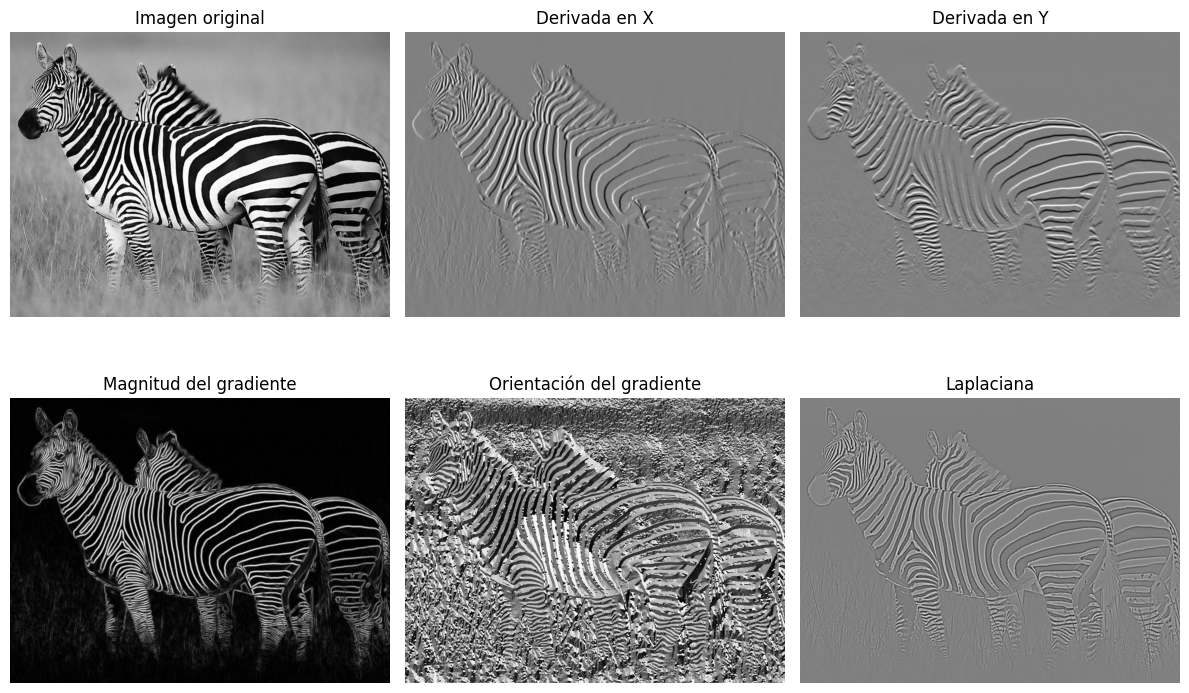
\includegraphics[width=1.0\textwidth, height=0.65\textwidth]{img/sin_titulo2.png}
    \caption{Resultado de la ejecución de la derivada en X, derivada en Y, magnitud del gradiente, orientación del gradiente y el Laplaciano de la imagen original}
    \label{fig:enter-label}
\end{figure}



 \noindent En efecto, atendiendo a dicha figura, comprobamos que:
\begin{itemize}
    \item Cuando derivamos con respecto a \textbf{x}, se realzan los bordes verticales ya que estamos buscando cambios abruptos de intensidad en el eje \textbf{x}. De manera análoga ocurre cuando derivamos con respecto a \textbf{y}, ya que lo que estamos haciendo es medir la tasa de variación de la intensidad en este eje detectando por tanto los bordes horizontales. Los bordes pueden ser blancos o negros, dependiendo de si ha habido un aumento o una disminución de intensidad.
    \item La magnitud del gradiente engloba ambas derivadas, y por eso podemos detectar tanto los bordes verticales como horizontales.
    \item La orientación del gradiente nos muestra información sobre la dirección en la que cambia la intensidad de la imagen.
    \item  El Laplaciano  combina contribuciones de ambas derivadas de segundo orden, lo que facilita la detección de bordes tanto verticales como horizontales. Esto lo convierte en una excelente opción para la detección de características.
\end{itemize}


\section{Núcleos de Sumabilidad}
La proposición \ref{prop:conv} afirma que $\mathscr{L}^1(\mathbb{R}^n)$ tiene estructura de anillo con respecto a las operaciones $+$ y $*$. Sin embargo, debemos notar que $\mathscr{L}^1(\mathbb{R}^n)$ carece de unidad. 

\noindent En efecto, supongamos que exista $K \in \mathscr{L}^1(\mathbb{R}^n)$ tal que se verificara 
\begin{equation}
    K * f = f * K = f \quad \forall f \in \mathscr{L}^1(\mathbb{R}^n).
\end{equation}
Entonces, tomando $f = G \in \mathscr{L}^1(\mathbb{R}^n)$, tenemos
\begin{equation}
   \widehat{K}(y)G(y) =  \widehat{K}(y)\widehat{G}(y) = G(y) \quad \forall y \in \mathbb{R}^n,
\end{equation}
de donde deducimos que necesariamente $\widehat{K}(y) = 1 \, \, \forall y \in \mathbb{R}^n$. Sin embargo, esto contradice el Lema de Riemann-Lebesgue.

\noindent Esta irregularidad no se presenta en el contexto discreto. Estudiaremos este hecho con mayor detenimiento en la segunda parte de la memoria. En ella, analizaremos el filtro impulso, que será aquel que, convolucionándolo con cualquier señal, resulte en ella misma. Vale la pena mencionar, en relación al análisis realizado en el capítulo anterior acerca de las operaciones de correlación y convolución, que este fenómeno no se manifiesta con la operación de correlación, marcando así una clara distinción entre ambas técnicas, y subrayando la convolución como una operación más intuitiva en términos de frecuencia, ya que proporciona una salida más natural.


\noindent No obstante, $\mathscr{L}^1(\mathbb{R}^n)$ cuenta con unidades aproximadas, denominadas núcleos de sumabilidad, que trataran de paliar los indeseados efectos provocados por la ausencia de unidad.

\noindent Previo a establecer de forma adecuadamente amplia el concepto de núcleo de sumabilidad, introducimos algunas definiciones.

\begin{definicion}
   Un \textit{conjunto dirigido} es un conjunto $\Lambda$ provisto de un orden $\leq$, tal que para cualesquiera $\lambda_1,\lambda_2 \in \Lambda$ existe $\mu \in \Lambda$ con $\lambda_1\leq \mu$ y  $\lambda_2\leq \mu$.
\end{definicion}

\begin{definicion}
   Una \textit{red} en un espacio topológico $X$ es una familia $\{x_{\lambda}\}_{\lambda \in \Lambda}$, donde $\Lambda$ es un conjunto dirigido.
\end{definicion}

\noindent Se dice que la red es convergente si existe $x \in X$ tal que para cada entorno $U$ de $x$ existe $\mu \in \Lambda$ tal que 
\begin{equation}
    \mu \in \Lambda, \mu \leq \lambda \implies x_{\lambda} \in U.
\end{equation}
\noindent Si $X$ es un espacio Hausdorff, entonces el punto $x$ es necesariamente único y se denota por $\lim_{\lambda \in \Lambda} \,$.


\begin{ejemplo}
Veamos algunos ejemplos para familiarizarnos con estas definiciones.
\begin{itemize}
    \item Tomamos como conjunto dirigido $\mathbb{N}_0$ con orden creciente, en cuyo caso 
    \begin{equation}
    \lim_{\lambda \in \Lambda} =     \lim_{n \rightarrow \infty}.
    \end{equation}
    \item Tomamos como conjunto dirigido $\mathbb{R}^+$ con orden decreciente, en cuyo caso 
    \begin{equation}
    \lim_{\lambda \in \Lambda} 
 = \lim_{\substack{t \rightarrow 0 \\ t > 0}}.
    \end{equation}
\end{itemize}
    
\end{ejemplo}

\noindent Definimos finalmente el concepto de núcleo de sumabilidad $\{K_{\lambda}\}_{\lambda \in \Lambda}$, que como puede intuir el lector poseerá la cualidad 
\begin{equation}
    \lim_{\lambda \in \Lambda} ||f*K-f||_1=0 \quad  \forall f \in \mathscr{L}^1(\mathbb{R}^n).
\end{equation}

\begin{definicion}\label{defnucl}
    Un\textit{ núcleo de sumabilidad} es una red $\{K_{\lambda}\}_{\lambda \in \Lambda}$ de funciones de $\mathscr{L}^1(\mathbb{R}^n)$ que verifica lo siguiente:
    \begin{itemize}
        \item para cada $\lambda \in \Lambda$,
        \begin{equation}
            \int_{\mathbb{R}^n} K_{\lambda}(x) \, dx = 1;
        \end{equation}

        \item existe una constante $M \in \mathbb{R}^+$ tal que, para cada $\lambda \in \Lambda$,
        \begin{equation}
            \int_{\mathbb{R}^n} |K_{\lambda}(x)| \, dx \leq M;
        \end{equation}
        \item  para cada $\delta \in \mathbb{R}^+$, se tiene que 
        \begin{equation}
            \lim_{\lambda \in \Lambda} \int_{||x|| > \delta} |K_{\lambda}(x)|\, dx = 0.
        \end{equation}
        
    \end{itemize}
\end{definicion}



\noindent A continuación, presentamos un resultado que proporciona una amplia gama de núcleos de sumabilidad.



\begin{proposicion}\label{consnuc}
Sea $K  \in \mathscr{L}^1(\mathbb{R}^n)$ tal que 
\begin{equation}
    \int_{\mathbb{R}^n}K(x) \, dx = 1
\end{equation}
y, para cada $\epsilon \in \mathbb{R}^+$, se define $K_{\epsilon}: \mathbb{R} \rightarrow \mathbb{C}$ por
\begin{equation}
    K_{\epsilon}(x) = \epsilon^{-n}K(\epsilon^{-1}x) \quad \forall x \in \mathbb{R}^n.
\end{equation}
Entonces la familia $\{K_{\epsilon}\}_{\epsilon \in \mathbb{R}^+}$ es un \textit{núcleo de sumabilidad}.
\end{proposicion}

\begin{proof}
Comprobaremos las condiciones que debe verificar un núcleo de sumabilidad. 
\begin{itemize}
    \item Para cada $\epsilon \in \mathbb{R}^+$, se tiene realizando un cambio de variable
    \begin{equation}
        \int_{\mathbb{R}^n}K_{\epsilon}(x) dx = \int_{\mathbb{R}^n} \epsilon^{-n}K(\epsilon^{-1}x) \, dx =  \int_{\mathbb{R}^n}K(x) \, dx = 1.
    \end{equation}
    \item   Para cada $\epsilon \in \mathbb{R}^+$, se tiene 
    \begin{equation}
        \int_{\mathbb{R}^n}|K_{\epsilon}(x)| dx = \int_{\mathbb{R}^n} \epsilon^{-n}|K(\epsilon^{-1}x)| \, dx =  \int_{\mathbb{R}^n}|K(x)| \, dx = ||K||_1.
    \end{equation}
    Por tanto, se verifica la segunda condición de la definición \ref{defnucl} con constante $M=||K||_1$.

    \item Fijamos un $\delta \in \mathbb{R}^+$, tenemos por tanto que
    \begin{equation}
        \int_{||x||>\delta} |K_{\epsilon}(x)| \, dx = \int_{||x||>\delta} \epsilon^{-n}|K(\epsilon^{-1}x)| \, dx = \int_{||x||>\delta/\epsilon} |K(x)| \, dx.
    \end{equation}
    Debemos entonces probar que 
    \begin{equation}
    \lim_{\substack{\epsilon \rightarrow 0 \\ \epsilon > 0}}\int_{||x||>\delta/\epsilon} |K(x)| \, dx  = 0.
    \end{equation}
    Para ello, vamos a usar el Teorema de la convergencia dominada.
    Sea $\{\epsilon_m\}$ una sucesión en $\mathbb{R}^+$ tal que $\{\epsilon_m\} \rightarrow 0$. Definimos una sucesión de funciones $\{\phi_m\} \in \mathscr{L}^1(\mathbb{R}^n)$ por
    \begin{equation}
        \phi_m(x) = 
    \begin{cases}
    |K(x)| & \text{si } ||x|| > \delta/\epsilon_m, \\
    0 & \text{si } ||x|| < \delta/\epsilon_m.
    \end{cases}
    \end{equation}
    Observamos que 
    \begin{equation}
        \int_{||x||> \delta/\epsilon_m} |K(x)|\, dx = \int_{\mathbb{R}^n} \phi_m(x) \, dx \quad \forall m \in \mathbb{N}.
    \end{equation}
    Aplicamos entonces el Teorema de la convergencia dominada a $\phi_m$.
    \begin{itemize}
        \item Como  $\{\delta/\epsilon_m\} \rightarrow 0$,
        \begin{equation}
            \lim_{m \rightarrow \infty} \phi_m(x) = 0 \quad \forall x \in \mathbb{R}^n.
        \end{equation}
        \item Se tiene que
        \begin{equation}
            |\phi_m(x)| \leq |K(x)| \quad \forall x \in \mathbb{R}^n, \forall m \in \mathbb{N},
        \end{equation}
        con $|K|$ integrable en $\mathbb{R}^n$.
    \end{itemize}
    Luego el Teorema de la convergencia dominada garantiza que 
    \begin{equation}
        \lim_{m \rightarrow \infty} \int_{\mathbb{R}^n} \phi_m(x) \, dx =0.
    \end{equation}
    De aquí deducimos que
     \begin{equation}
    \lim_{m \rightarrow \infty }\int_{||x||>\delta/\epsilon_m} |K(x)| \, dx  = 0,
    \end{equation}
    cumpliéndose así la última condición.
    
\end{itemize}
Concluimos que para cada $ \epsilon \in \mathbb{R}^+$ la familia $\{K_{\epsilon}\}_{\epsilon \in \mathbb{R}^+}$ es un núcleo de sumabilidad.
\end{proof}



\begin{ejemplo}[Núcleo de Gauss-Weierstrass]
    La familia de funciones $\{G_t\}_{t\downarrow
0}$ definida por
    \begin{equation}
        G_{t}: \mathbb{R}^n \rightarrow \mathbb{R}, \, G_{t}(x) = \frac{1}{(4 \pi t)^{-n/2}}e^{- \pi ||x||^2} \quad \forall x \in \mathbb{R}^n, \forall t \in \mathbb{R}^+,
    \end{equation}
    se denomina \textit{núcleo de Gauss-Weierstrass}.
    
    \vspace{0.1cm}
    \noindent Observamos que este núcleo es la familia de funciones $\{K_{\sqrt{4\pi t}}\}_{t \in \mathbb{R}^+}$ asociada a la proposición \ref{consnuc}, con $K = G \in \mathscr{L}^1(\mathbb{R}^n)$.
\end{ejemplo}

\begin{definicion}\label{gauss}
    Definimos $P : \mathbb{R}^n \rightarrow \mathbb{R}$ función de $  \mathscr{L}^1(\mathbb{R}^n)$ dada por
    \begin{equation}
        P(x) =  C_n \frac{1}{(1 + ||x||^2)^{\frac{n+1}{2}}}, \; \; \; \text{con} \, \, C_n = \frac{\Gamma({\frac{n+1}{2}})}{\pi^{\frac{n+1}{2}}}
    \end{equation}
    y donde $\Gamma$ es la función gamma.
\end{definicion}

\begin{lema}\label{lem:leam}
$P$ cumple
\begin{equation}\label{loq}
    \int_{\mathbb{R}^n} P(x)\, \, dx = 1 .
\end{equation}
\end{lema}
\begin{proof}

Comprobaremos que se verifica
\begin{equation}
        \frac{1}{C_n} = \int_{\mathbb{R}^n} \frac{1}{(1 + ||x||^2)^{\frac{n+1}{2}}} \,dx,
\end{equation}
que es equivalente a~\eqref{loq}.

\noindent Usamos coordenadas polares:
\[
\int_{\mathbb{R}^n} \frac{1}{(1 + ||x||^2)^{\frac{n+1}{2}}} \, dx \,  = w_{n-1}\int_{0}^{\infty} \frac{r^{n-1}}{(1+r^2)^{\frac{n+1}{2}}} dr,
\]
donde $w_{n-1}$ denota el área de $\mathbb{S}^{n-1}$.

\noindent Aplicamos el cambio de variable, \(r = \tan(\theta)\), y obtenemos
\begin{align}
 w_{n-1}\int_{0}^{\infty} \frac{r^{n-1}}{(1+r^2)^{\frac{n+1}{2}}} dr &=  w_{n-1}\int_{0}^{\pi/2} \frac{(\tan(\theta))^{n-1}}{(1+(\tan(\theta))^2)^{\frac{n+1}{2}}} (1+ \tan(\theta))^2 d\theta \\
 &=  w_{n-1}\int_{0}^{\pi/2} \frac{(\tan(\theta))^{n-1}(\cos(\theta))^{n+1}}{(\cos(\theta))^2} d\theta \\
 &=  w_{n-1}\int_{0}^{\frac{\pi}{2}} (\sin(\theta))^{n-1} d\theta.
\end{align}

\noindent Realizando el cambio de variable $u = (\sin(\theta))^2$, resulta
\[
w_{n-1}\int_{0}^{\frac{\pi}{2}} (\sin(\theta))^{n-1} d\theta =  \frac{1}{2}w_{n-1}\int_{0}^{1} (1-s)^{\frac{n}{2}-1}s^{\frac{1}{2}-1} ds = \frac{1}{2}w_{n-1}\beta\left(\frac{n}{2},\frac{1}{2}\right).
\]
Sustituyendo ahora el valor de $w_{n-1}$ y utilizando la relación de la función beta $\beta$ con la función gamma $\Gamma$, se tiene:
\[
 w_{n-1}\beta\left(\frac{n}{2},\frac{1}{2}\right)= \frac{2 \Gamma\left(\frac{n}{2}\right) \Gamma\left(\frac{1}{2}\right)}{\Gamma\left(\frac{n+1}{2}\right)} = \frac{\pi^{\frac{n+1}{2}}}{\Gamma\left(\frac{n+1}{2}\right)}.
\]
Concluimos que
\begin{equation*}
\int_{\mathbb{R}^n} \frac{1}{(1 + ||x||^2)^{\frac{n+1}{2}}} \, dx =
\frac{\pi^{\frac{n+1}{2}}}{\Gamma\left(\frac{n+1}{2}\right)} = \frac{1}{C_n}.  \qedhere
\end{equation*}
 
\end{proof}


\begin{ejemplo}[Núcleo de Poisson]
    La familia de funciones $\{P_y\}_{y\downarrow
0}$ definida por
    \begin{equation}
        P_{y}: \mathbb{R}^n \rightarrow \mathbb{R}, \; \; \; \, P_{y}(x) = C_n \frac{y}{(y^2 + ||x||^2)^{\frac{n+1}{2}}}, \; \; \; \; \text{con} \, \, C_n = \frac{\Gamma({\frac{n+1}{2}})}{\pi^{\frac{n+1}{2}}},
    \end{equation}
    se denomina \textit{núcleo de Poisson}.

    \noindent Observamos que este núcleo es la familia de funciones $\{K_{y}\}_{y \in \mathbb{R}^+}$ asociada a la proposición \ref{consnuc} con $K = P \in \mathscr{L}^1(\mathbb{R}^n)$.
\end{ejemplo}

\begin{lema}\label{lema:previo}
    Sea $K  \in \mathscr{L}^1(\mathbb{R}^n)$ tal que 
\begin{equation}
    \int_{\mathbb{R}^n}K(x) \, dx = 1.
\end{equation}
Supongamos $1 \leq p < \infty$, y $f \in \mathscr{L}^p(\mathbb{R}^n)$. Entonces
\begin{equation}
|| f*K_{\lambda}-f||_p \leq \int_{\mathbb{R}^n} w_pf(x) |K_{\lambda}(x)| \, dx.
\end{equation}
\end{lema}
\begin{proof}
\noindent Para cada  $x \in \mathbb{R}^n$ tal que $(f*K)(x)$ está definida, tenemos 
 \begin{align}
    |(f*K)(x)-f(x)| &= \left|\int_{\mathbb{R}^n}f(x-t)K(t) \, dt - f(x) \int_{\mathbb{R}^n}K(t) \,dt \right| \\
    &\leq \int_{\mathbb{R}^n} \left|f(x-t)-f(x) \right| |K(t)| \, dt. \\ 
\end{align}
\noindent Distinguimos dos casos:
\begin{itemize}
    \item Suponemos que $p=1$. Usando el Teorema de Tonelli, tenemos que
    \begin{align*}
        ||f*K-f||_1 &= \int_{\mathbb{R}^n} |(f*K_{\lambda})(x)-f(x)| \, dx\\
        &\leq \int_{\mathbb{R}^n} \int_{\mathbb{R}^n} \left|f(x-t)-f(x) \right| |K_{\lambda}(t)| \, dt \, dx \\
        &= \int_{\mathbb{R}^n} \int_{\mathbb{R}^n} \left|f(x-t)-f(x) \right| |K(t)| \, dx \, dt  =\int_{\mathbb{R}^n} w_1f(t) |K(t)|\, dt.
    \end{align*}
    \item Suponemos que $1<p<\infty$. Tomamos $q = \frac{p}{p-1}$, de modo que $\frac{1}{p}+\frac{1}{q}=1$.
    Aplicando el Teorema de Tonelli de nuevo, obtenemos
    \begin{align}
    ||f*K-f||_p^p &= \int_{\mathbb{R}^n}|(f*K_{\lambda})(x)-f(x)|^p \, dx  =  \\
    &\leq \int_{\mathbb{R}^n} |(f*K_{\lambda})(x)-f(x)||(f*K_{\lambda})(x)-f(x)|^{p-1} \, dx. \\ 
    &\leq \int_{\mathbb{R}^n} \left(\int_{\mathbb{R}^n} \left|f(x-t)-f(x) \right| |K(t)| \, dt \right)|(f*K_{\lambda})(x)-f(x)|^{p-1} \, dx. \\ 
    &\leq \int_{\mathbb{R}^n} \left(\int_{\mathbb{R}^n} \left|f(x-t)-f(x) \right| |(f*K_{\lambda})(x)-f(x)|^{p-1} \,dx \right) |K(t)|\, dt. \\ 
\end{align}
    Ahora aplicamos la desigualdad de H\"{o}lder 
    \begin{align}
    &\int_{\mathbb{R}^n} \left(\int_{\mathbb{R}^n} \left|f(x-t)-f(x) \right| |(f*K_{\lambda})(x)-f(x)|^{p-1} \,dx \right) \\
    &\leq \left( \int_{\mathbb{R}^n} \left|f(x-t)-f(x) \right|^p \, dx  \right)^{1/p} \left( \int_{\mathbb{R}^n} |(f*K_{\lambda})(x)-f(x)|^{(p-1)q} \, dx  \right)^{1/q} \\
    &\leq \left( \int_{\mathbb{R}^n} \left|f(x-t)-f(x) \right|^p \, dx  \right)^{1/p} \left( \int_{\mathbb{R}^n} |(f*K_{\lambda})(x)-f(x)|^{p} \, dx  \right)^{1/q}  \\
    &= w_pf(t)||f*K-f||_p^{p/q}.
\end{align}
\noindent De donde deducimos que 
\begin{equation}
       ||f*K-f||_p^p \leq \int_{\mathbb{R}^n} w_pf(t)||f*K-f||_p^{p/q} |K(t)|\, dt = ||f*K-f||_p^{p/q}\int_{\mathbb{R}^n} w_pf(t) |K(t)|\, dt,
\end{equation}
\noindent luego 
\begin{equation}
       ||f*K-f||_p \leq \int_{\mathbb{R}^n} w_pf(t) |K(t)|\, dt.
\end{equation}
\end{itemize}
En ambos casos se verifica la desigualdad. 
\end{proof}






\begin{teorema} \label{teo:suma}
    Sea $\{K_{\lambda}\}_{\lambda \in \Lambda}$ un núcleo de sumabilidad. Supongamos $1 \leq p < \infty$, y $f \in \mathscr{L}^p(\mathbb{R}^n)$. Entonces
    \begin{equation}
        \lim_{\lambda \in \Lambda} ||f*K_{\lambda}-f||_p=0.
    \end{equation}
\end{teorema}
\begin{proof}
Fijamos $\delta \in \mathbb{R}^+$, para cada $\lambda \in \Lambda$, usando el Lema \ref{lema:previo}, se tiene que
\begin{align}
    || f*K_{\lambda}-f||_p &\leq \int_{\mathbb{R}^n} w_pf(x) |K_{\lambda}(x)| \, dx \\
    &= \int_{||x|| < \delta} w_pf(x) |K_{\lambda}(x)| \, dx +\int_{||x|| > \delta} w_pf(x) |K_{\lambda}(x)| \, dx.
\end{align}
\noindent Analizamos cada uno de los sumandos por separado. Para el primero, usamos que $K_{\lambda}$ es un núcleo de sumabilidad:
\begin{equation}
    \int_{||x|| < \delta} w_pf(x) |K_{\lambda}(x)| \, dx \leq \sup_{||x|| < \delta}w_pf(x)\int_{||x|| < \delta} |K_{\lambda}(x)| \, dx  \leq M\sup_{||x|| < \delta}w_pf(x).
\end{equation}
\noindent Y, por otro, usando la proposición \ref{mod_cont}, sabemos que
\begin{equation}
    \int_{||x|| > \delta} w_pf(x) |K_{\lambda}(x)| \, dx \leq 2 ||f||_p\int_{||x|| > \delta} |K_{\lambda}(x)| \, dx.
\end{equation}

\noindent Juntando ambas acotaciones,   
\begin{equation}
     || f*K_{\lambda}-f||_p \leq M\sup_{||x|| < \delta}w_pf(x)+ 2 ||f||_p\int_{||x|| > \delta} |K_{\lambda}(x)| \, dx.
\end{equation}
Luego
\begin{equation}
    \limsup_{\lambda \in \Lambda}|| f*K_{\lambda}-f||_p \leq M\sup_{||x|| < \delta}w_pf(x).
\end{equation}
Esto es válido para todo $\delta \in \mathbb{R}^+$, por lo que 
\begin{equation}
    \lim_{\delta \rightarrow 0}\sup_{||x|| < \delta}w_pf(x)= 0.
\end{equation}
En consecuencia
\begin{equation}
    \limsup_{\lambda \in \Lambda}|| f*K_{\lambda}-f||_p =0,
\end{equation}
concluyendo que 
\begin{equation*}
    \lim_{\lambda \in \Lambda}|| f*K_{\lambda}-f||_p =0.\qedhere
\end{equation*}
\end{proof}


\begin{corolario} \label{coro:coro}
    Sea $K  \in \mathscr{L}^1(\mathbb{R}^n)$ tal que 
    \begin{equation}
        \int_{\mathbb{R}^n}K(x) \, dx = 1.
    \end{equation}
    Para cada $\epsilon \in \mathbb{R}^+$, se define $K_{\epsilon}: \mathbb{R} \rightarrow \mathbb{C}$ por
    \begin{equation}
        K_{\epsilon}(x) = \epsilon^{-n}K(\epsilon^{-1}x) \quad \forall x \in \mathbb{R}^n.
    \end{equation}
     Supongamos $1 \leq p < \infty$, y $f \in \mathscr{L}^p(\mathbb{R}^n)$. Entonces
    \begin{equation}
        \lim_{\substack{\epsilon \rightarrow 0 \\ \epsilon > 0}} ||f* K_{\epsilon}-f||_p=0.
    \end{equation}
\end{corolario}


\begin{proof}
    Basta con usar el Teorema \ref{teo:suma}, y la Proposición \ref{consnuc}.
\end{proof}




\begin{teorema} \label{contnuc}
    Sea $\{K_{\lambda}\}_{\lambda \in \Lambda}$ un núcleo de sumabilidad, y $f \in \mathscr{L}^{\infty}(\mathbb{R}^n)$.
    \begin{itemize}
        \item Supongamos que $f$ es continua en cada punto de un subconjunto compacto $E \subset \mathbb{R}^n$. Entonces
        \begin{equation}
            \lim_{\lambda  \in \Lambda} \max_{x \in E} |(f*K_{\lambda})(x)-f(x)|=0.
        \end{equation}
        En particular, si $f$ es continua en un punto $x \in \mathbb{R}^n$,
         \begin{equation}\label{punt}
            \lim_{\lambda  \in \Lambda} (f*K_{\lambda})(x)=f(x).
        \end{equation}
        \item Supongamos que $f$ es uniformemente continua en $\mathbb{R}^n$. Entonces
        \begin{equation}
            \lim_{\lambda  \in \Lambda} ||(f*K_{\lambda})(x)-f(x)||_{\infty}=0.
        \end{equation}
    \end{itemize}
\end{teorema}
\begin{proof}
    Como $f \in \mathscr{L}^{\infty}(\mathbb{R}^n)$, sabemos que la convolución $f*K_\lambda$ está definida en todo $\mathbb{R}^n$ y está acotada. Dado $\epsilon \in \mathbb{R}^+$, notemos los siguientes puntos: 
    \begin{itemize}
    
        \item Por la continuidad de $f$ en cada punto del conjunto compacto $E$, se tiene que $\exists \delta \in \mathbb{R}^+$ tal que 
        \begin{equation}
            x \in E, \, ||x-t||< \delta \implies |f(x-t)-f(x)| < \frac{\epsilon}{2M}.
        \end{equation}
        
        \item Al ser $\{K_{\lambda}\}_{\lambda \in \Lambda}$ un núcleo de sumabilidad, existe $ M >0$ tal que para todo $ \lambda \in \Lambda$
        \begin{equation}
             \int_{\mathbb{R}^n} |{K_\lambda}(x)| \, dx \leq M.
        \end{equation}
        Además, también existe $ \mu \in \Lambda$ tal que
        \begin{equation}
            \lambda \in \Lambda, \mu \leq \lambda \implies 2 ||f||_\infty   \int_{||x|| > \delta} |K_{\lambda}(x)|\, dx < \frac{\epsilon}{2}.
        \end{equation} 
    \end{itemize}

    \noindent Para $\lambda \in \Lambda$ con $ \mu \leq \lambda$, y para cada $x \in E$, usando los puntos anteriores, se tiene que
    
     \begin{align*}
        |(f*K_{\lambda})(x)-f(x)| &= \left|\int_{\mathbb{R}^n}f(x-t)K_{\lambda}(t) \, dt - f(x) \int_{\mathbb{R}^n}K_{\lambda}(t) \,dt \right| \\
        &\leq \int_{\mathbb{R}^n} \left|f(x-t)-f(x) \right| |K_{\lambda}(t)| \, dt \\
        &=   \int_{||t|| < \delta} \left|f(x-t)-f(x) \right| |K_{\lambda}(t)| \, dt + \int_{||t|| > \delta} \left|f(x-t)-f(x) \right| |K_{\lambda}(t)| \, dt \\ 
        &\leq \frac{\epsilon}{2M}\int_{||t|| < \delta}  |K_{\lambda}(t)| \, dt + 2 ||f||_\infty\int_{||t|| > \delta} |K_{\lambda}(t)| \, dt 
        \leq \frac{\epsilon}{2M}M + \frac{\epsilon}{2} = \epsilon.
    \end{align*}


    \noindent Por tanto,
    
    \begin{equation}
        \max_{x \in E} |(f*K_{\lambda})(x)-f(x)| \leq \epsilon.
    \end{equation}
    Finalmente, si $f$ es continua en un punto $x \in \mathbb{R}^n$, tomando como conjunto compacto $E = \{x\}$, se sigue que 
    \begin{equation*}\label{punt}
            \lim_{\lambda  \in \Lambda} (f*K_{\lambda})(x)=f(x).\qedhere
        \end{equation*}
\end{proof}


\begin{corolario}  \label{coro2}
    Sea $K  \in \mathscr{L}^1(\mathbb{R}^n)$ tal que 
    \begin{equation}
        \int_{\mathbb{R}^n}K(x) \, dx = 1.
    \end{equation}
    Para cada $\epsilon \in \mathbb{R}^+$, se define $K_{\epsilon}: \mathbb{R} \rightarrow \mathbb{C}$ por
    \begin{equation}
        K_{\epsilon}(x) = \epsilon^{-n}K(\epsilon^{-1}x) \quad \forall x \in \mathbb{R}^n.
    \end{equation}
     Sea también $f \in \mathscr{L}^{\infty}(\mathbb{R}^n)$.
    \begin{itemize}
        \item Supongamos que $f$ es continua en cada punto de un subconjunto compacto $E \subset \mathbb{R}^n$. Entonces
        \begin{equation}
            \lim_{\substack{\epsilon \rightarrow 0 \\ \epsilon > 0}} \max_{x \in E} |(f*K_{\epsilon})(x)-f(x)|=0.
        \end{equation}
        En particular, si $f$ es continua en un punto $x \in \mathbb{R}^n$,
         \begin{equation}
            \lim_{\substack{\epsilon \rightarrow 0 \\ \epsilon > 0}} (f*K_{\epsilon})(x)=f(x).
        \end{equation}
        \item Supongamos que $f$ es uniformemente continua en $\mathbb{R}^n$. Entonces
        \begin{equation}
           \lim_{\substack{\epsilon \rightarrow 0 \\ \epsilon > 0}} ||(f*K_{\epsilon})(x)-f(x)||_{\infty}=0.
        \end{equation}
    \end{itemize}
\end{corolario}


\begin{proof}
    Basta con usar el Teorema \ref{contnuc}, y la proposición \ref{consnuc}.
\end{proof}

\begin{observacion}
    Cabe mencionar que en el segundo apartado del Teorema \ref{contnuc} y el Corolario \ref{coro2} se exige que la función $f$ sea uniformemente continua, y esta condición no es caprichosa. En efecto, como hemos anotado anteriormente, al estar $f \in \mathscr{L}^{\infty}(\mathbb{R}^n)$, se tiene que  para todo $\lambda \in \Lambda, \, \,\,  f*K_{\lambda}$ es uniformemente continua en $\mathbb{R}^n$, por lo que si se cumple que
    \begin{equation}
            \lim_{\lambda  \in \Lambda} ||(f*K_{\lambda})(x)-f(x)||_{\infty}=0,
    \end{equation}
    se tiene que necesariamente $f$ es uniformemente continua en $\mathbb{R}^n$.
\end{observacion}


\noindent

\section{Métodos de Sumación}

Retomamos en esta sección el desafío de reconstruir una función $f \in \mathscr{L}^1(\mathbb{R}^n)$ a partir de su Transformada de Fourier $\widehat{f}$. El lector puede pensar que este objetivo ya se alcanzó mediante  el Teorema de Inversión. Sin embargo, para su aplicación, se  obligaba a que necesariamente la función Transformada fuera integrable en $\mathbb{R}^n$ (de hecho, si no lo era, no tenía sentido la reconstrucción planteada en~\eqref{eq:teoinv}). Sin embargo, como ya comentamos en el primer capítulo, esta es una hipótesis ciertamente restrictiva, y es por ello por lo que se plantean otras posibles interpretaciones para reconstruir la función.

\vspace{0.5cm}
\noindent Recordamos los métodos se sumabilidad de las series de Fourier, que consistían en la utilización de las sumas ponderadas 
\begin{equation}
    \sum_{k=-\infty}^{\infty}\widehat{f}(k)e^{ikx}\Phi(\epsilon k),
\end{equation}
donde $\Phi$ era una función de peso adecuada y la ejecución del límite en $\epsilon = 0$ de éstas.
Parece natural tratar de utilizar en nuestra situación integrales ponderadas
\begin{equation}
 \int_{\mathbb{R}^n}\widehat{f}(y)e^{2\pi i \langle x, y \rangle} \Phi(\epsilon y) \, dy 
\end{equation}
y ejecutar el límite en $\epsilon = 0$. 

\begin{proposicion} \label{ame}
    Sea $\Phi \in \mathscr{L}^1(\mathbb{R}^n)$ tal que
    \begin{equation}
        \Phi(-x) = \Phi(x) \quad \forall x \in \mathbb{R}^n,
    \end{equation}
y pongamos $K = \widehat{\Phi}$. Para cada $ \epsilon \in \mathbb{R}^+$, se define la función $K_{\epsilon}: \mathbb{R} \rightarrow \mathbb{C}$ por
\begin{equation}
    K_{\epsilon}(x) = \epsilon^{-n}K(\epsilon^{-1}x) \quad \forall x \in \mathbb{R}^n.
\end{equation}
Supongamos $f \in \mathscr{L}^1(\mathbb{R}^n)$. Entonces se verifica
\begin{equation}\label{eq:c }
     \int_{\mathbb{R}^n}\widehat{f}(y)e^{2\pi i \langle x, y \rangle} \Phi(\epsilon y) \, dy  = (f*K_{\epsilon})(x) \quad \forall x \in \mathbb{R}^n, \forall \epsilon \in \mathbb{R}^+.
\end{equation}
\end{proposicion}

\begin{proof}
   \noindent Comenzamos anotando los siguientes hechos: 
   \begin{itemize}
       \item Por un lado, sabemos que la función $y \mapsto \widehat{f}(y)e^{2\pi i \langle x, y \rangle} \Phi(\epsilon y)$ es el producto de una función continua y acotada $y \mapsto \widehat{f}(y)e^{2\pi i \langle x, y \rangle}$ por una función integrable   $y  \mapsto \Phi(\epsilon y)$.
       \item Como $K$ es la Transformada de Fourier de una función integrable en $\mathbb{R}^n$, sabemos que está acotada en $\mathbb{R}^n$. Luego también lo está $K_{\epsilon}$, y eso hace que la convolución $f*K_{\epsilon}$ esté definida en todo $\mathbb{R}^n$.
       \item Como $\Phi(x) = \Phi(-x) \quad \forall x \in \mathbb{R}^n$, se sigue que $K(x) = K(-x)$, y entonces $K_{\epsilon}(x) = K_{\epsilon}(-x) \quad \forall x \in \mathbb{R}^n, \, \forall \epsilon \in \mathbb{R}^+.$
   \end{itemize}
   \item Fijamos $x \in \mathbb{R}^n$ y $\epsilon \in \mathbb{R}^+$. Se tiene que
  \begin{equation*}
    \begin{aligned}
      \int_{\mathbb{R}^n} \widehat{f}(y)e^{2 \pi i \langle x,y \rangle}\Phi(\epsilon y) \, dy
        &= \int_{\mathbb{R}^n} \widehat{\tau_{-x}f}(y)H_{\epsilon}\Phi(y) \, dy 
        = \int_{\mathbb{R}^n} \tau_{-x}f(y) \widehat{H_{\epsilon}\Phi}(y) \, dy \\
        &= \int_{\mathbb{R}^n} \tau_{-x}f(y)\epsilon^{-n}\widehat{\Phi}(\epsilon^{-1}y) \, dy 
        = \int_{\mathbb{R}^n} \tau_{-x}f(y)K_{\epsilon}(y) \, dy \\
        &= \int_{\mathbb{R}^n} f(x+y)K_{\epsilon}(y) \, dy 
        = \int_{\mathbb{R}^n} f(x-y)K_{\epsilon}(-y) \, dy \\
        &= \int_{\mathbb{R}^n} f(x-y)K_{\epsilon}(y) \, dy 
        = (f * K_{\epsilon})(x).
    \end{aligned}
\end{equation*}
Por tanto, hemos probado~\eqref{eq:c}.
\end{proof}


\begin{lema}\label{lema}
Sea $\Phi \in \mathscr{L}^1{(\mathbb{R}^n)}$ y supongamos que se cumplen las siguientes condiciones:
\begin{itemize}
    \item $\Phi$ es continua en $0$, 
    \item $\Phi(0) = 1$,
    \item $\widehat{\Phi} \in \mathscr{L}^1(\mathbb{R}^n).$
\end{itemize}
Entonces, 
\begin{equation}
    \int_{\mathbb{R}^n} \widehat{\Phi}(y) \, dy = 1.
\end{equation}
\end{lema}

\begin{proof}
    Basta con aplicar el Teorema de Inversión a $\Phi$, cuya Transformada es integrable en $\mathbb{R}^n$. Como $\Phi $ es continua en $0$, se tiene que 
    \begin{equation}
        1 = \Phi(0) = \int_{\mathbb{R}^n} \widehat{\Phi}(y) \, dy.
    \end{equation}
\end{proof}

\begin{teorema}\label{teoteo}
    Sea $\Phi \in \mathbb{R}^n$ y suponemos que se verifica que
    \begin{itemize}
         \item $\Phi$ es continua en $0$, 
    \item $\Phi(0) = 1$,
    \item $\widehat{\Phi} \in \mathscr{L}^1(\mathbb{R}^n).$
    \end{itemize}
    Si $f \in \mathscr{L}^1(\mathbb{R}^n)$, entonces
    \begin{equation}
        \lim_{\substack{\epsilon \rightarrow 0 \\ \epsilon > 0}} \int_{\mathbb{R}^n} \left| f(x) -   \int_{\mathbb{R}^n}\widehat{f}(y)e^{2\pi i \langle x, y \rangle} \Phi(\epsilon y) \, dy \right| \, dx = 0.
    \end{equation}
\end{teorema}
\begin{proof}
Sea $K = \widehat{\Phi}$. Por un lado, sabemos por la proposición \ref{ame}  que 
\begin{equation}\label{eq:c }
     \int_{\mathbb{R}^n}\widehat{f}(y)e^{2\pi i \langle x, y \rangle} \Phi(\epsilon y) \, dy  = (f*K_{\epsilon})(x) \quad \forall x \in \mathbb{R}^n, \forall \epsilon \in \mathbb{R}^+.
\end{equation}
\noindent Por otra parte, sabemos que por el Lema \ref{lema} se cumple que 
\begin{equation}
    \int_{\mathbb{R}^n} K(x) \, dx = 1.
\end{equation}
\noindent Por tanto, aplicando el Corolario \ref{coro:coro} se tiene que 
\begin{equation*}
    0 = \lim_{\substack{\epsilon \rightarrow 0 \\ \epsilon > 0}}||f-f*K_{\epsilon}||_1  = \lim_{\substack{\epsilon \rightarrow 0 \\ \epsilon > 0}} \int_{\mathbb{R}^n} \left| f(x) -   \int_{\mathbb{R}^n}\widehat{f}(y)e^{2\pi i \langle x, y \rangle} \Phi(\epsilon y) \, dy \right| \, dx = 0. \qedhere
\end{equation*}
\end{proof}
\begin{teorema}\label{teoteoteo}
    Sea $\Phi \in \mathbb{R}^n$ y suponemos que se verifica que
    \begin{itemize}
         \item $\Phi$ es continua en $0$, 
    \item $\Phi(0) = 1$,
    \item $\widehat{\Phi} \in \mathscr{L}^{\infty}(\mathbb{R}^n).$
    \end{itemize}
    Si $f \in \mathscr{L}^{\infty}(\mathbb{R}^n)$, entonces
    \begin{itemize}
        \item Supongamos que $f$ es continua en cada punto de un subconjunto compacto $E \subset \mathbb{R}^n$. Entonces
        \begin{equation}
             \lim_{\substack{\epsilon \rightarrow 0 \\ \epsilon >0}}\int_{\mathbb{R}^n}\widehat{f}(y)e^{2\pi i \langle x, y \rangle} \Phi(\epsilon y) \, dy  = f(x)
        \end{equation}
        uniformemente en $E$, esto es, 
         \begin{equation}
        \lim_{\substack{\epsilon \rightarrow 0 \\ \epsilon > 0}} \max_{x \in E}  \left| f(x) -   \int_{\mathbb{R}^n}\widehat{f}(y)e^{2\pi i \langle x, y \rangle} \Phi(\epsilon y) \, dy \right|  = 0.
    \end{equation}
    En particular, si $f$ es continua en un punto $x \in \mathbb{R}^n$, entonces
    \begin{equation}
             \lim_{\substack{\epsilon \rightarrow 0 \\ \epsilon > 0}}\int_{\mathbb{R}^n}\widehat{f}(y)e^{2\pi i \langle x, y \rangle} \Phi(\epsilon y) \, dy  = f(x). 
        \end{equation}

    \item  Si $f$ es uniformemente continua en $\mathbb{R}^n$, entonces
    \begin{equation}
              \lim_{\substack{\epsilon \rightarrow 0 \\ \epsilon >0}}\int_{\mathbb{R}^n}\widehat{f}(y)e^{2\pi i \langle x, y \rangle} \Phi(\epsilon y) \, dy  = f(x)
        \end{equation}
        uniformemente en $\mathbb{R}^n$,
        esto es, 
         \begin{equation}
        \lim_{\substack{\epsilon \rightarrow 0 \\ \epsilon > 0}} \sup_{x \in \mathbb{R}^n}  \left| f(x) -   \int_{\mathbb{R}^n}\widehat{f}(y)e^{2\pi i \langle x, y \rangle} \Phi(\epsilon y) \, dy \right|   = 0.
    \end{equation}
    \end{itemize}
\end{teorema}
\begin{proof}
Sea $K = \widehat{\Phi}$. Por un lado sabemos por la proposición \ref{ame}  que 
\begin{equation}\label{eq:c }
     \int_{\mathbb{R}^n}\widehat{f}(y)e^{2\pi i \langle x, y \rangle} \Phi(\epsilon y) \, dy  = (f*K_{\epsilon})(x) \quad \forall x \in \mathbb{R}^n, \forall \epsilon \in \mathbb{R}^+.
\end{equation}
\noindent Por otra parte, sabemos que por el Lema \ref{lema} se cumple que 
\begin{equation}
    \int_{\mathbb{R}^n} K(x) \, dx = 1.
\end{equation}
Además,
\begin{equation}
    |K(x)| = |\widehat{\Phi}(x)| \leq ||\Phi||_1 \quad \forall x \in \mathbb{R}^n.
\end{equation}
\noindent El Corolario \ref{contnuc} proporciona el resultado deseado.
\end{proof}
\begin{observacion}
   Es posible prescindir de la condición de $ f \in \mathscr{L}^{\infty}(\mathbb{R}^n)$ con una teoría más extensa sobre los núcleos de sumabilidad. Este aspecto se reserva para trabajo futuro.
\end{observacion}

\subsection{Método de Sumación de Gauss}

Sea $f \in \mathscr{L}^1(\mathbb{R}^n).$ El\textit{ método de sumación de Gauss} consiste en utilizar el límite
\begin{equation}
     \lim_{\substack{\epsilon \rightarrow 0 \\ \epsilon > 0}} \int_{\mathbb{R}^n}\widehat{f}(y)e^{2\pi i \langle x, y \rangle} e^{-\epsilon ||y|| ^2} \, dy
\end{equation}
como mecanismo de inversión de la Transformada de Fourier de $f$.

\noindent Para cada $\epsilon \in \mathbb{R}^+$ y cada  $x \in \mathbb{R}^n$, se tiene que
\begin{equation}
    \int_{\mathbb{R}^n}\widehat{f}(y)e^{2\pi i \langle x, y \rangle} e^{-\epsilon ||y|| ^2} \, dy = \int_{\mathbb{R}^n}\widehat{f}(y)e^{2\pi i \langle x, y \rangle} G\left(\frac{\sqrt{\epsilon}}{\sqrt{\pi}}y\right) \, dy. 
\end{equation}

\noindent Sabemos que 
\begin{itemize}
    \item $G \in \mathscr{L}^1(\mathbb{R}^n)$,
    \item $G$ es continua en $\mathbb{R}^n$,
    \item $G(0)=1$,
    \item $G(x)=G(-x)$,
    \item $\widehat{G}=G \in \mathscr{L}^1(\mathbb{R}^n)$.
\end{itemize}

\begin{corolario}
    Si $f \in \mathscr{L}^1(\mathbb{R}^n)$, entonces
    \begin{equation}
        \lim_{\substack{\epsilon \rightarrow 0 \\ \epsilon > 0}} \int_{\mathbb{R}^n} \left| f(x) -   \int_{\mathbb{R}^n}\widehat{f}(y)e^{2\pi i \langle x, y \rangle} e^{-\epsilon ||y||^2} \, dy \right| \, dx = 0.
    \end{equation}
\end{corolario}
\begin{proof}
    El resultado se deduce del Teorema \ref{teoteo}, tomando $\Phi = G$ y como $\epsilon$ tomamos $\frac{\sqrt{\epsilon}}{\sqrt{\pi}}$.
\end{proof}


\begin{teorema}

    Sea $f \in \mathscr{L}^{\infty}(\mathbb{R}^n)$.
    \begin{itemize}
        \item Supongamos que $f$ es continua en cada punto de un subconjunto compacto $E \subset \mathbb{R}^n$. Entonces
        \begin{equation}
             \lim_{\substack{\epsilon \rightarrow 0 \\ \epsilon >0}}\int_{\mathbb{R}^n}\widehat{f}(y)e^{2\pi i \langle x, y \rangle} e^{-\epsilon ||y||^2} \, dy  = f(x) 
        \end{equation}
        uniformemente en $E$, esto es, 
         \begin{equation}
        \lim_{\substack{\epsilon \rightarrow 0 \\ \epsilon > 0}} \max_{x \in E}  \left| f(x) -   \int_{\mathbb{R}^n}\widehat{f}(y)e^{2\pi i \langle x, y \rangle} e^{-\epsilon ||y||^2} \, dy \right|  = 0.
    \end{equation}
    En particular, si $f$ es continua en un punto $x \in \mathbb{R}^n$, entonces
    \begin{equation}
             \lim_{\substack{\epsilon \rightarrow 0 \\ \epsilon > 0}}\int_{\mathbb{R}^n}\widehat{f}(y)e^{2\pi i \langle x, y \rangle} e^{-\epsilon ||y||^2} \, dy  = f(x). 
        \end{equation}

    \item  Si $f$ es uniformemente continua en $\mathbb{R}^n$, entonces
    \begin{equation}
              \lim_{\substack{\epsilon \rightarrow 0 \\ \epsilon >0}}\int_{\mathbb{R}^n}\widehat{f}(y)e^{2\pi i \langle x, y \rangle} e^{-\epsilon ||y||^2} \, dy  = f(x)
        \end{equation}
        uniformemente en $\mathbb{R}^n$,
        esto es, 
         \begin{equation}
        \lim_{\substack{\epsilon \rightarrow 0 \\ \epsilon > 0}} \sup_{x \in \mathbb{R}^n}  \left| f(x) -   \int_{\mathbb{R}^n}\widehat{f}(y)e^{2\pi i \langle x, y \rangle} e^{-\epsilon ||y||^2} \, dy \right|   = 0.
    \end{equation}
    \end{itemize}
\end{teorema}


\begin{proof}
    El resultado se deduce del Teorema \ref{teoteoteo}, tomando $\Phi = G$ y como $\epsilon$ tomamos $\frac{\sqrt{\epsilon}}{\sqrt{\pi}}$.
\end{proof}











